\chapter{Heavy $\to$ Heavy Meson Semileptonic Decays}
\label{chap:semileptonic}

In this chapter we will review the key physical principles and theoretical machenery one needs to understand semileptonic decays involving heavy quarks. The presence of hadrons in these processes neccessitates an introduction to strong interaction physics. The presence of heavy quarks offers us extra theoretical leverage to divide and conquer the different relevant scales of the decays.

\section{Strong Interaction Physics}
\label{sec:stronginteractions}

It has been pretty much established that the strong interaction, and the observed pattern of hadrons, can be explained with a non-abelian Yang-Mills field and a number of flavours of fermions (quarks) that interact with it [SO MUCH EVIDENCE]. In this section we review the main features of the fundemental theory, along with a useful effective theory for describing dynamics at the hadron level. 

\subsection{Quantum Chromodynamics}

{\red{

    qcd lagrangian, symmetries, asymptotic freedom

}}

Quantum Chromodynamics (QCD) is defined to be the $SU(3)$ Yang-Mills gauge theory. The Lagrangian is derived by requiring:
\begin{itemize}
\item
  $N_f$ fermion fields transforming in the fundemental representation of  an $SU(3)$ gauge group.
\item
  Invariance under that gauge group.
\item
  Renormalizability of all interactions.
\end{itemize}
From these we find \cite{Schwartz:2013pla}
\begin{align}
  \mathscr{L}_{\text{QCD}} &= \sum_f \bar{q}_f (i \slashed{D} - m_f) q_f - {1\over 4} \text{Tr}G_{\mu\nu} G^{\mu\nu} - g{\bar{\theta}\over 64 \pi^2} \epsilon^{\mu\nu\rho\sigma} \text{Tr}G_{\mu\nu} G_{\rho\sigma} \\
  &D_{\mu} = \partial_{\mu} - i g G_{\mu} \\
  &G_{\mu\nu} = [ D_{\mu}, D_{\nu} ]
\end{align}
$q_f = ( q_{f,r}, q_{f,b}, q_{f,g} )$ are the $N_f$ fermions, transforming under $q_f(x) \to U(x)q_f(x)$, $\bar{q}_f(x) \to \bar{q}_f(x) U^{\dagger}(x)$ where $U(x)$ is an $SU(3)$ matrix. $G_{\mu}$ are the $\mathfrak{su}(3)$-valued gluon fields, transforming under $G_{\mu}(x) \to U(x) G_{\mu}(x) U^{\dagger}(x) - i/g [ \partial_{\mu} U(x) ] U^{\dagger}(x)$. $g$ is the coupling constant of the theory, often expressed instead as $\alpha_s = (g/4\pi)^2$. $\bar{\theta}$ has strong experimental bounds on it's size, to the extent for our purposes it can be neglected \cite{ALTAREV1992242}.
\\ \\
The most notable feature of QCD is due to the running of the QCD coupling $\alpha_s$ \cite{PhysRevLett.30.1343}.
\begin{figure}
  \begin{center}
    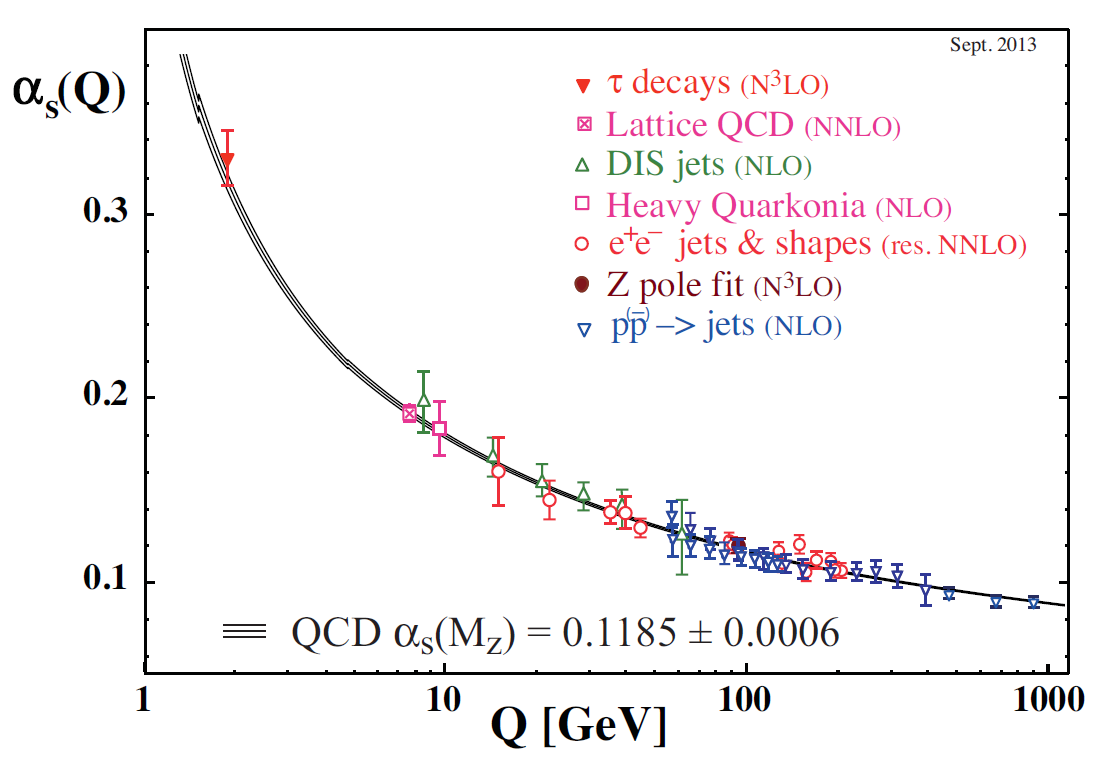
\includegraphics[width=0.7\textwidth]{images/QCD-running-coupling.png}
  \end{center}
  \caption{The relationship between scale $Q$ and the strong coupling constant $\alpha_s$, from the Particle Data Group \cite{Patrignani:2016xqp}}
  \label{fig:semileptonic}
\end{figure}
In contrast with the electroweak force, the coupling of the strong force diverges at low energies. This is referred to as {\it{asymptotic freedom}}. At energies at and below $\Lqcd \sim 0.3$GeV, $\alpha_s$ becomes too large to be a good expansion parameter, and perturbation theory becomes unreliable for making predictions.
\\ \\
At large $\alpha_s$, quarks and gluons become strongly interacting, this is beleived to be the source of confinement, the mechanism that bounds quarks together into hadrons. A common assumption then is that all of the dynamics that occurs inside hadrons have energies on the scale of $\Lqcd$.
\\ \\
We arrive at the conclusion that processes involving hadrons cannot be understood using the traditional method of perturbation theory. Broadly speaking there are two alternative approaches:
\begin{enumerate}
\item
  Chiral Perturbation theory - an effective theory of hadrons with the same symmetry properties as QCD. This will be introduced in the next section.
\item
  Lattice simulations - solve the path integral by brute force, eliminating the need for an expansion in $\alpha_s$. This is covered in sections \ref{chap:latticeqcd} and \ref{chap:latticecalculations}, since it is the method used in the work presented in this thesis.
\end{enumerate}

\subsection{Chiral Symmetry}

{\red{

    chiral symmetry, spontanious SB,

    explicit SB

    WARD IDENTITIES
    
    chiral pert. theory, pion octet.

}}

In the limit of $m_f\to 0,\forall f$, QCD develops two new global symmetries between the flavours;
\begin{align}
  q_f(x) &\to \exp(i\theta_a \lambda^{ff'}_a) q_{f'}(x) \\
  q_f(x) &\to \exp(i\gamma_5 \theta_a \lambda^{ff'}_a) q_{f'}(x)
\end{align}
where $\lambda_a$ are $U(N_f)$ matrices. They are labelled $U(N_f)_V$ and $U(N_f)_A$ respectively, standing for vector and axial. {\color{red}{Each of these groups can be decomposed into $U(1)_{V/A}\times SU(N_f)_{V/A}$, the $U(1)$ contains the single element corresponding to $\lambda_a=1$, and $SU(N_f)$ contains the elements where $\lambda_a$ are $SU(N_f)$ generators. Neccesary?}} In the below we will take $N_f=3$ when discussing physical aspects of the symmetry, since in the regeime where chiral symmetry is important, the heavier three quarks do not effect the dynamics.
\\ \\
Via Noether's theorem, these symmetries imply currents that are conserved in the massless limit \cite{Scherer:2002tk};
\begin{align}
    \label{eq:vectorcurrent}
  V_{\mu}^a &= \bar{q} \gamma_{\mu} \lambda_a q \quad,\quad \partial^{\mu}V_{\mu}^a = i \bar{q} [ M, \lambda_a ] q \\
  A_{\mu}^a &= \bar{q} \gamma_{\mu} \gamma_5 \lambda_a q \quad,\quad \partial^{\mu}A_{\mu}^a = i \bar{q} \{ M, \lambda_a \}\gamma_5 q
  \label{eq:axialcurrent}
\end{align}
where $M = \text{diag}(m_u,m_d,m_s,...)$ acts on flavour. Since one can connect any two flavours via the $U(N_f)$ generators, one can build such currents charged with any combination of flavours from linear combinations of \eqref{eq:vectorcurrent},\eqref{eq:axialcurrent}, i.e.
\begin{align}
	\label{eq:individualflavs1}
	V_{\mu}^{ff'} &= \bar{q}_f \gamma_{\mu} q_{f'} \quad,\quad \partial^{\mu}V_{\mu}^{ff'} = i (m_f - m_{f'}) S_{ff'} \\
	  A_{\mu}^{ff'} &= \bar{q}_f \gamma_{\mu} \gamma_5 q_j \quad,\quad \partial^{\mu}A_{\mu}^{ff'} = i (m_f+m_{f'})P_{ff'}
	\label{eq:individualflavs2}
\end{align}
where $S_{ff'} = \bar{q}_f q_{f'}$, $P_{ff'} = \bar{q}_f \gamma_5 q_{f'}$ are the scalar and pseudoscalar densities. The non-conservation equations in \eqref{eq:individualflavs1},\eqref{eq:individualflavs2} are examples of Ward identities.
\\ \\
A useful theorem \cite{Fubini:1964boa} is that partially conserved currents (currents that become conserved when some parameter in the theory vanishes, like $V_{\mu}^{ff'}$ and $A_{\mu}^{ff'}$) require no renormalization. This comes in useful when matching operators between regularization schemes, and will be used in {\color{red}{chapter N}}.
\\ \\
\subsubsection{Spontanious Chiral Symmetry Breaking}

Besides the explicit breaking of chiral symmetry by the quark masses, the $U(N_f)_A$ symmetry is also {\it{spontaniously broken}} by the QCD dynamics. This is to say that, while the Lagrangian still holds this symmetry, the ground state of the theory is not invariant under such transformations;
\begin{align}
  Q_A^a | 0 \rangle \neq 0
  \label{eq:chiralssb}
\end{align}
where $Q_A^a = \int d^3x A_0^a(x)$ is the conserved charge associated with the axial symmetry, and therefore also the generator of that symmetry acting on the Hilbert space \cite{Scherer:2002tk}.
\\ \\
There are three pieces of evidence for this claim.
\begin{itemize}
\item
  Scalar quark condensate. Using the comutation relations of $U(N_f)_A$, and assuming $Q_V^a | 0 \rangle = 0$, one can show that \eqref{eq:chiralssb} implies
  \begin{align}
    \langle 0 | \bar{u} u | 0 \rangle = \langle 0 | \bar{d} d | 0 \rangle = \langle 0 | \bar{s} s | 0 \rangle \neq 0
  \end{align}
  This value has been calculated in \cite{PhysRevD.87.034503} to be $\sim 290$GeV.
\item
  Lack of Parity Doubling. $Q^a_A$ transforms states to states with opposite parity. If $Q^a_A$ was unbroken we could say that $[Q_A^a,H]=0$ ($H$ is the Hamiltonian), and from this demonstrate a degeneracy between states of opposite parity that interact with the strong force, for example a degeneracy between scalar and pseudoscalar particles. However, Pseudoscalar particles are not even approximately degenerate to scalar particles \cite{Patrignani:2016xqp}.
\item
  The Light Pseudoscalar Octet. Goldstone's theorem says that for every spontaniously broken generator, there should be a massless spin-zero excitation with the same quantum numbers as that generator (Goldstone boson). In the case of $N_f=3$, 8 the broken $Q_A^a$'s would lead to an octet of massless pseudoscalar particles. In the presence of explicit symmetry breaking by the quark masses, these pseudoscalars would not be massless but have small masses proportional to the quark masses (pseudo-Goldstone bosons). This is exactly what is observed: there is an octet of pions, kaons and $\eta$ particles that have masses ($\sim 200$MeV) much lower than any other states in QCD (e.g. the $\rho$ meson, with mass $\sim 1$GeV) {\color{red}{ref!}}.
\end{itemize}
\subsubsection{Chiral Perturbation Theory ($\chi$PT)}

Chiral Perturbation Theory is an effective theory of the pseudo-Goldstone bosons in the massless limit. It is useful for lattice calculations as it gives us information about how observables in strongly interacting systems should vary with light quark mass. This can be used when extrapolations in light quark masses are performed. It is also a useful language for understanding finite volume effects in lattice simulations, since a finite volume will effect the lightest degrees of freedom in the system.
\\ \\
Terms in $\chi$PT are organized by number of derivatives acting on the fields, since we assume the excitations to have small masses (proportional to light quark masses), and are approximately on-shell.
\\ \\
Goldstone's theorem tells us that the (pseudo-)Goldstone bosons should have the same transformation properties under the chiral symmetry as the broken generators, in our case those of $SU(3)_A$. Using this, and the requirement that the theory should be $SU(3)_V$ invariant, we can write down the leading order Lagrangian (minimal number of derivatives):
\begin{align}
  \label{eq:chipt}
  \mathscr{L}_2 = {f^2\over 4} \text{Tr}[ \partial_{\mu} U \partial^{\mu}U^{\dagger} ] \\
  U = \exp\left( {i\over f} \sum_{a=1}^8 \lambda_a \phi_a \right)
\end{align}
$\lambda_a$ are $SU(3)$ generators and $\phi_a$ are the eight Goldstone bosons.
\\ \\
Connections between $\chi$PT and QCD can be found by considering how extrernal fields interact with either of the theories. For example, one can consider the quark masses in QCD as external scalar fields which couple to scalar currents $\bar{q}_f q_f$ and obtain a vev. One then asks: how would this field have to transform under the chiral symmetry for QCD to be $SU(3)_V$ invariant? So we are imagining $M=\text{diag}(m_u,m_d,m_s,...)$ is a field that transforms like
\begin{align}
  M \to \exp(i(1-\gamma_5)\theta_a\lambda_a) M \exp(-i(1+\gamma_5)\theta_b\lambda_b)
\end{align}
One then transitions into $\chi$PT and asks: what interactions between the Goldstone fields and $M$ are allowed by $SU(3)_V$? The answer is
\begin{align}
  \mathscr{L}_M = {f^2 B_0 \over 2} \text{Tr}[ MU^{\dagger} + U M^{\dagger} ]
\end{align}
where $B_0$ is a new parameter of the theory. By comparing ground state energies of the two theories, i.e. $\langle 0 | H_{\text{QCD}} | 0 \rangle = \langle 0 | H_{\chi\text{PT}} | 0 \rangle$, one can identify $B_0 = \langle \bar{u}u \rangle/f^2$. By expanding $\mathscr{L}_M$ in powers of quark masses and $1/f$, one can find mass terms for the Goldstones. Three of the goldstones are mass eigenstates, with masses given by
\begin{align}
  &M_{\pi^0}^2 = B_0 ( m_u + m_d ) \\
  &M_{K^0}^2 = B_0 \left( {1\over2} m_u + {1\over2} m_d + m_s \right) \\
  &M_{\eta}^2 = {2\over3}B_0 \left( {1\over2} m_u + {1\over2} m_d + 2m_s \right)
\end{align}
where $\pi$,$K$, and $\eta$ correspond to the physical mesons $\pi,K,\eta$, since their masses approximately respect these relations. Other terms that come out of expanding $\mathscr{L}_{M}$ become mixing terms between the $\phi_a$'s, via these we can identify the rest of the fields with physical mesons, resulting in
\begin{align}
  &\pi^0 = \phi_3 \quad\quad K^0/\bar{K}^0 = (\phi_6 \pm i\phi_7)/\sqrt{2} \quad\quad \eta = \phi_8 \\
  &\pi^{\pm} = (\phi_1 \pm i \phi_2)/\sqrt{2} \quad\quad K^{\pm} = (\phi_4 \pm i\phi_5 )/\sqrt{2}
  \nonumber
\end{align}
By a similar process one can deduce the Chiral currents in $\chi$PT, for example the axial current is given by $A_{\mu}^a = i f^2\text{Tr}[ \lambda_a ( U^{\dagger} \partial_{\mu} U - (\partial_{\mu} U) U^{\dagger} )]/4$. By computing $\langle 0 | A^3_{\mu} | \pi^0 \rangle = M_{\pi^0} f_{\pi^0}$, one can identify the parameter $f$ to be equal to the Pion decay constant $f_{\pi^0}$ at leading order in $\chi$PT.
\\ \\
Predictions in $\chi$PT can be systematically improved by including terms with more derivatives in $\mathscr{L}_{\chi\text{PT}}$.


\section{Heavy Quark Physics}

Quarks with mass $m_Q >> \Lqcd$ are referred to as heavy quarks. Charm and bottom quarks are considered heavy: $\Lqcd/m_c \sim 1/4$, $\Lqcd/m_b \sim 1/14$. This separation of scales can come in very useful. They mean one can integrate out the degrees of freedom at $m_Q$, and still have a good description of the dynamics at $\Lqcd$. As will be demonstrated, this does not mean totally removing the heavy quark from the theory.
\\ \\
The physical picture of a meson containing a heavy quark is very similar to that of a hydrogen atom. In the hydrogen atom, the nucleus has a mass much greater than the charactoristic energies of the electron and photons. One can treat the nucleus as a static source of electric charge, and solve to high precision the dynamics of the electron. The electron's behaviour is not affected by the mass or the spin of the nucleus. Similarly, one can consider a heavy quark in a meson to be a static source of color charge, and solve the $\Lqcd$ dynamics in it's presence. The mass and spin of the heavy quark does not effect the light degrees of freedom, this is the well understood {\it{heavy quark symmetries}}. The effective field theories introduced in this section gives us a framework to take this approximation and systematically correct for it.

\subsection{HQET}

{\red{

    derivation of leading order HQET

    form factors in HQET, isgur-wise function

    luke's theorem

}}

Heavy Quark Effective Theory (HQET) is an effective field theory with the cutoff at the heavy quark mass $m_Q$, and terms organized in a series in $\Lambda_{\text{QCD}}/m_Q$. Since at the $b$ (and $c$) mass QCD is perturbative ($\alpha_s(m_Q) << 1$), one can match HQET to perturbative QCD at $m_Q$, then run the couplings of HQET down to produce useful predictions at the confinement scale.
\\ \\
It is a useful tool for when we perform extrapolations in heavy quark mass, as it supplies us with explicit expressions for the heavy quark mass dependance on various phenomenological quantities.

\subsubsection{HQET Lagrangian}

As a simple example, we will derive HQET for a single heavy quark interacting with gluons. The fermion part of the Lagrangian is
\begin{align}
	\mathscr{L}_{\text{QCD}} = \bar{Q} ( i\slashed{D} - m_Q ) Q,
	\label{eq:dirac}
\end{align}
where $Q$ is the heavy quark field. Define the heavy quark velocity $v$ according to
\begin{align}
	v = {p_Q \over m_Q}.
\end{align}
Now split $Q$ into "heavy" and "light" components:
\begin{align}
	\label{eq:hdef}
	Q = h + H\quad : \quad &h = {1\over 2} e^{-im_Q v\cdot x} ( 1 + \slashed{v} ) Q \\
	&H = {1\over 2} e^{-im_Q v\cdot x} ( 1 - \slashed{v} ) Q
\end{align}
with the important property
\begin{align}
	\slashed{v} h = h \quad \slashed{v} H = - H.
\end{align}
In terms of these new fields the Lagrangian becomes
\begin{align}
	\mathscr{L}_{\text{QCD}} = i\bar{h} (v\cdot D) h - \bar{H} ( i(v\cdot D) - 2m_Q ) H 
		+ i \bar{h} \slashed{D}^{\perp} H + i \bar{H} \slashed{D}^{\perp} h.
		\label{eq:HQET_preintegral}
\end{align}
where $v_{\mu}(v\cdot D)$ is the covariant derivative projected along the direction of $v$, and $D^{\perp} = D - v_{\mu}(v\cdot D)$ is the components perpendicular to $v$. In the rest frame of the heavy quark, $v = (1,0,0,0)$ so $v_{\mu}(v\cdot D)$ becomes the temporal derivative and $D^{\perp}$ the spacial. The physical interpretation of the above definition can be seen by acting a spacial derivative on the definition of $h$, and by recognising $\partial Q = -i p_Q$, $\partial h = -i p_h$, we find that
\begin{align}
	p_Q = m_Q v + p_h
\end{align} 
Since $p_h << p_Q$, we see that the quark's momentum is dominated by it's mass (the quark is close to on-shell), and the $h$ field represents perturbations around on-shell due to interactions with the lighter degrees of freedom at $\Lambda_{\text{QCD}}$.
\\ \\
From \eqref{eq:HQET_preintegral}, we see that $h$ is a massless field and $H$ has a mass of $2m_Q$. From this Lagrangian we can derive an equation of motion for $H$:
\begin{align}
	( i(v\cdot D) + 2m_Q) H = i\slashed{D}^{\perp} h,
\end{align}
with the solution
\begin{align}
	H = {1\over i(v\cdot D) + 2m_Q} i\slashed{D}^{\perp} h = {1\over 2m_Q}\sum_{n=0}^{\infty} {(-i(v\cdot D))^n\over 2m_Q} \slashed{D}^{\perp} h.
\end{align}
By substituting this into the Lagrangian we arrive at
\begin{align}
	\mathscr{L}_{\text{HQET}} = i \bar{h} (v\cdot D) h - \bar{h} \slashed{D}^{\perp} {1\over 2m_Q}\sum_{n=0}^{\infty} {(-i(v\cdot D))^n\over 2m_Q} \slashed{D}^{\perp} h.
\end{align}
This can be found by a more rigorous proof by performing the Gaussian integration over the $H$ field in the path integral {\color{red}{ref!}}. Since we expect $v\cdot D \sim \Lambda_{\text{QCD}}$, we can interpret the infinite sum as a series in $\Lambda_{QCD}/m_Q$, and truncate it at some order. For example to $\mathcal{O}(\Lambda_{\text{QCD}}/m_Q)$, we have
\begin{align}
	\mathcal{L}_{\text{HQET}^1} = i \bar{h} (v\cdot D) h - {1\over 2m_Q} \bar{h} \slashed{D}^{\perp 2} h
	\label{eq:HQET1}
\end{align}
 Leading order HQET exhibits new symmetries not present in full QCD, known as the heavy quark symmetries. Since $m_Q$ is not present in the leading order Lagrangian, there is a flavour symmetry - a set of $N$ heavy quarks with the same $v$ can be mixed via an $SU(N)$ symmetry. Similarly due to the absense of spin mixing matrices, a heavy quark has an $SU(2)$ spin symmetry. This builds up a physical picture of a heavy quark in a meson being a static colour charge, the dynamics at $\Lambda_{\text{QCD}}$ is not effected by it's mass or spin.

\subsubsection{Isgur-Wise Function}
\label{sec:isgurwise}

A consequence of heavy quark symmetry relevant to semileptonic decays are the Wigner-Eckart theorems. Consider a transition amplitude between two heavy pseudoscalar mesons:
\begin{align}
	\langle M(v) | \bar{h} \Gamma h | M(v') \rangle
\end{align}
The spin structure of $| M(v) \rangle$ is $\gamma_5 (1-\slashed{v})$, this can be shown with the following argument. The state can be generally written as $| M(v) \rangle = \int d^4x d^4y f(x,y) \bar{h}(x) \gamma_5 q(y) | \Omega \rangle$ which, using $\slashed{v} h = h$, can be reexpressed as $| M(v) \rangle = \int d^4x d^4y f(x,y) \bar{h}(x) \gamma_5 (1-\slashed{v}) q(y) | \Omega \rangle /2$. Then via the spin symmetry, one can always rotate the $h$ spin in the meson state such that it matches the spin of the current, i.e. $h_{\alpha} \bar{h}_{\beta} \to 1_{\alpha\beta} f(h,\bar{h})$. Then the amplitude can be written as
\begin{align}
	\langle M(v) | \bar{h} \Gamma h | M(v') \rangle = m_M Tr[ {1\over 2} \gamma_5 (1 - \slashed{v}) \Gamma {1\over 2} \gamma_5 (1 - \slashed{v'}) \mathcal{M}(v,v')]
	\label{eq:wignereckart1}
\end{align} 
where $\mathcal{M}(v,v')$ can be any gamma-matrix valued function. The $m_M$ factor comes from the relativistic normalization of the states. A general spin decomposition of this is
\begin{align}
	\mathcal{M}(v,v') = \xi_0(v\cdot v') + \slashed{v} \xi_1(v\cdot v') + \slashed{v'} \xi_2(v\cdot v') + \slashed{v}\slashed{v'} \xi_4(v\cdot v').
\end{align}
Plugging this into \eqref{eq:wignereckart1}, we can then write the amplitude in terms of a single function:
\begin{align}
\langle M(v) | \bar{h} \Gamma h | M(v') \rangle = m_M Tr[ {1\over 2} \gamma_5 (1 - \slashed{v}) \Gamma {1\over 2} \gamma_5 (1 - \slashed{v'}) ] \xi(v\cdot v')
\end{align}
where $\xi(v\cdot v') = \xi_0(v\cdot v') + \xi_1(v\cdot v') - \xi_3(v\cdot v') - \xi_4(v\cdot v')$ is known as the Isgur-Wise function. For a general pair of mesons with spin structure $\mathcal{H}$,$\mathcal{H}'$, a transition amplitude between them with a heavy current insertion can always be written as
\begin{align}
	\langle \mathcal{H} | \bar{h} \Gamma h | \mathcal{H}' \rangle = \xi(v\cdot v') Tr[ \bar{\mathcal{H}} \Gamma \mathcal{H} ] + \order{\Lambda_{\text{QCD}}\over m_Q}
\end{align}
So all heavy semileptonic decays involving any combination of masses or spins are described by a single non-perturbative function, $\xi(v\cdot v')$. A couple of relevant examples are:
\begin{align}
	\langle D(v') | \bar{c_{v'}} \gamma^{\mu} b_v | \bar{B}(v) \rangle = \sqrt{m_B m_D} ( v + v')^{\mu} \xi(v\cdot v') \\
	\langle D^*(v') | \bar{c_{v'}} \gamma^{\mu} b_v | \bar{B}(v) \rangle = i \sqrt{m_B m_D*} \epsilon^{\mu\nu\alpha\beta} \varepsilon_{\nu}^* v'_{\alpha} v_{\beta} \xi(v\cdot v')  \\
	\langle D^*(v') | \bar{c_{v'}} \gamma^{\mu}\gamma_5 b_v | \bar{B}(v) \rangle = \sqrt{m_B m_D*} [ \varepsilon^{*\mu}(v\cdot v' + 1) - v^{'\mu} \varepsilon^*\cdot v] \xi(v\cdot v').
\end{align}
Here we have subscripted the fields $c_{v'}$,$b_v$ to specify the velocity used to separate those fields from the heavy components e.g. in eq. \eqref{eq:hdef}. 

\subsubsection{AG and Luke's Theorem}

Luke's theorem, which can be derived from the Ademollo-Gatto (AG) theorem, tells us the leading order heavy quark mass dependance of form factors. First we will derive the AG theorem. We will follow the proof given in \cite{Lebed:1991sq}.
\\ \\
Consider the transition amplitude
\begin{align}
	\langle \alpha | Q_a | \beta \rangle
\end{align}
where $Q_a$ is a conserved charge associated with some global symmetry $\mathcal{G}$, and $|\alpha\rangle$ and $|\beta\rangle$ belong to an irrep of $\mathcal{G}$. Imagine explicitly breaking the symmetry with a term like $\mathscr{L}_{\text{break}} = \lambda \mathcal{O}_{\text{break}}$. The states in the broken theory can be expressed as
\begin{align}
	|\beta \rangle = c_{\beta\beta} | \beta' \rangle + \sum_{m} c_{\beta m} | m' \rangle \\
	\langle \alpha | = c^*_{\alpha\alpha} \langle \alpha' | + \sum_{n} c^*_{\alpha n} \langle n' |.
\end{align}
where primed states are states belonging to irreps of $\mathcal{G}$. Here $|m'\rangle$ can only be states that can be mixed with $| \beta \rangle$ by $\mathcal{O}_{\text{break}}$ via the broken dynamics of the theory, and similarly for $\langle n' |$ and $\langle \alpha |$. The transition amplitude becomes
\begin{align}
\nonumber
	\langle \alpha | Q_a | \beta \rangle
	 	&= c_{\alpha\alpha}^* c_{\beta\beta} \langle \alpha' | Q_a | \beta' \rangle \\ 
	 	\nonumber
	 	&+ \sum_m c_{\alpha\alpha}^* c_{\beta m} \langle \alpha' | Q_a | m' \rangle \\
	 	\nonumber 
	 	&+ \sum_n c_{\alpha n}^* c_{\beta \beta} \langle n' | Q_a | \beta \rangle \\ 
	 	&+ \sum_m\sum_n c_{\alpha n}^* c_{\beta m} \langle n' | Q_a | m' \rangle
	 	\label{eq:AGproofexpanded}
\end{align}
The theorem applies to the situation where $|n'\rangle$ and $|m'\rangle$ live in different $\mathcal{G}$ irreps to $|\alpha\rangle$ and $|\beta \rangle$ (we assume $|\alpha\rangle$ and $|\beta \rangle$ to be in the same irrep otherwise the transition amplitude will always be zero). In this case the amplitudes in the second and third terms vanish. Now consider the order of the coefficients $c_{nm}$. We can assume that $c_{nm} = \order{\lambda}$ for arbitrary $n,m \neq \alpha,\beta$, since switching off the symmetry breaking by setting $\lambda=0$ should cause $|\alpha\rangle $ and $|\alpha'\rangle$ to coencide. Then, using the normalization of the states $\sum_{n} |c_{\alpha n} |^2 = 1$, we find $c_{\alpha\alpha} = \sqrt{1 - \order{\lambda}^2} = 1 + \order{\lambda^2}$, and similarly for $c_{\beta\beta}$. Applying this to the two surviving terms in \eqref{eq:AGproofexpanded}, we end up with
\begin{align}
	\langle \alpha | Q_a | \beta \rangle = 1 + \order{\lambda^2}
\end{align}
This is the AG theorem: if the current $Q_a$ and the symmetry breaking therm $mathcal{O}$ act orthogonally on the states, the transition amplitude can have at most a second order correction in the symmetry breaking parameter.
\\ \\
Now we will apply this to HQET to produce Luke's theorem. Consider a transition including two heavy quarks ($b$ and $c$). Then, the heavy quark symmetry is a spin symmetry for each flavour, and a flavour symmetry between them. The leading order spin symmetry breaking terms can be found from \eqref{eq:HQET1} to be
\begin{align}
	{1\over 4m_Q} \bar{h} \gamma^{\mu} \gamma^{\nu} F_{\mu\nu} h 
\end{align}
for both $h=b$ and $h=c$. The leading order flavour breaking term is
\begin{align}
	\left({1\over 2m_b} - {1\over 2m_c} \right) {1\over 2} \bar{h} \sigma_z \slashed{D}^{\perp 2} h
\end{align}
where now $h = (b,c)$ and the $\sigma_z$ is the third pauli matrix acting on flavour. These terms cause states, for example $| B \rangle$ to mix with states $|n'\rangle$, each being of the order of at least one of the following: $1/2m_b$,$1/2m_c$, and $(1/2m_b - 1/2m_c)$. It can be shown (\cite{Lebed:1991sq}) that the leading order symmetry breaking terms can only mix pseudoscalar and vector mesons with other irreps of the heavy quark symmetries. Hence, for example the example of the $B \to D$ transition, where
\begin{align}
	\langle D | \bar{c}\gamma_{\mu} b | B \rangle &= 1 + \order{\epsilon_b^2} 
	+ \order{\epsilon_c^2} \\ &+ \order{\left( \epsilon_b - \epsilon_c \right)^2}.
\end{align}
where we have now defined $\epsilon_h = 1/2m_h$. This implies the Isgur-Wise function $\xi$ also has corrections of this order. As we move away from the infinite-mass limit, $\xi$ becomes $h_+$, and $h_-$ becomes non-zero. In this case we see that
\begin{align}
	h_+(q^2_{\text{max}}) &= ( 1 + \order{ \epsilon_b^2}
	+ \order{\epsilon_c^2} \\ &+ \order{\left( \epsilon_b - \epsilon_c \right)^2} ) \\
	h_-(q^2_{\text{max}}) &= ( \order{ \epsilon_b }
	+ \order{ \epsilon_c } + \order{ \epsilon_b - \epsilon_c } )
\end{align}
Away from $q^2_{\text{max}}$, the velocities for the $b$ and $c$ quarks become different, resulting in a new flavour breaking term in the effective Lagrangian;
\begin{align}
	i \bar{c} (v - v')\cdot D c \sim \order{1-{E_D\over M_D}} + \order{ \underline{p}_D/\over M_D }
\end{align}
where to deduce the orders we took the rest frame of the $B$ meson. This results in extra corrections of these orders (raised to the second power) in the form factors. 

\subsubsection{Second Order Form Factors}

The process in \ref{sec:isgurwise} of decomposing matrix elements into general expressions parameterized by non-perturbative functions can be extended beyond leading order in HQET. In \cite{Falk:1992wt} this process was continued to second order in $1/m_b$ and $1/m_c$ for $B\to D^{(*)}$ transitions. The form factors for general $v,v'$ that are relevant to our work, were found to have the forms
\begin{align}
	h_+ &= \xi + (\epsilon_b + \epsilon_c ) L_1 + ( \epsilon_b^2 + \epsilon_c^2 ) l_1 + \epsilon_b \epsilon_c \phi_1 \\
	h_- &= ( \epsilon_c - \epsilon_b )L_4 + (\epsilon_c^2-\epsilon_b^2) l_4\\
	h_{A_1} &= \xi + \epsilon_c  L_{25} + \epsilon_b L_{14} + \epsilon_c^2 l_{25} + \epsilon_b^2 l_{14} + \epsilon_c\epsilon_b \phi_2
\end{align}
where, due to the normalization of the form factors for $m_c=m_b$ at $q^2_{\text{max}}$;
\begin{align}
L_1(q^2_{\text{max}}) = L_{25}(q^2_{\text{max}}) = L_{14}(q^2_{\text{max}}) = 0
\end{align}
A calculation using the non-relativistic constituent quark model \cite{PhysRevD.39.799} estimates the factor $l_1(q^2_{\text{max}}) = -3m_q^2$ where $q$ is the spectator of the decay.

\subsubsection{Decay Constants}

{\color{red}questions that still need answered: \\ 
1) how come the $\sqrt{m_b}$ from state normalizations don't appear in $h_+$ etc?
2) how much does the above stuff apply away from continuum limit? }

\subsection{NRQCD}

{\red{

    NRQCD motivation

    'derivation' of NRQCD

    foldy-wouthousiousen transform

}}

An effective field theory closely related to HQET is Non-Relativistic QCD (NRQCD). This differs from HQET only by the power couting; instead of organizing terms in the Lagrangian according to their order in $\Lambda_{\text{QCD}}/m$, the terms are organized in terms of orders of the heavy quark's spacial velocity $v \sim p/m$ (where now $p=|\underline{p}|$). NRQCD is derived with the following process:
\begin{itemize}
\item
Separate the quark and antiquark components of the heavy quark $Q$. Define the antiquark-free 2-component spinor $h$ via $Q = e^{\underline{\gamma}\cdot \underline{\nabla}/2m}\begin{pmatrix} h\\ 0 \end{pmatrix}$ \cite{PhysRev.78.29}.
\item
Define power-counting by considering the expected expectation values of operators for heavy mesons \cite{Lepage:1992tx}. The three relevant scales concerning the heavy meson are $M$,$p\sim Mv$ and $E_K\sim Mv^2$, where $M$ is the meson mass, $p$ the spacial momentum and $E_K$ the kinetic energy. By relating operators to these three scales, we deduce their order in $v$. Start with the normalization of a scalar current:
\begin{align}
	\langle M | \int d^3x h^{\dagger}(x) h(x) | M \rangle \sim 1
	\label{eq:nrqcd_scalarnormalization}
\end{align}
where $| M \rangle$ is some heavy meson state. Since we expect the meson state to be localized in a region of size $1/p$, we can assert that
\begin{align}
	\int d^3x \sim {1\over p^3}
\end{align}
from this and \eqref{eq:nrqcd_scalarnormalization}, we find $h \sim p^{3/2} \sim v^{3/2}$. 
The order of the derivative operator can be deduced from
\begin{align}
	E_K = \langle M | \int d^3x h^{\dagger}(x) {\underline{D}^2\over 2M} h(x) | M \rangle
\end{align}
to be $D \sim v$. Following such a chain of arguments, we can deduce the order in $v$ of any operator.

\item
The Lagrangian to $\order{v^n}$ is then simply all of the operators satisfying the symmetries of $QCD$ of orders below $v^n$, with some Wilson coefficients \cite{Lepage:1992tx}. To $\order{v^6}$:
\begin{align}
\nonumber
	&\mathscr{L}_{\text{NRQCD}} = h^{\dagger} \Bigg( i D_0 + {\underline{D}^2 \over 2m} + c_1 {\underline{D}^4\over m^3}
	+ c_2 g{\underline{D}\cdot \underline{E} - \underline{E} \cdot \underline{D} \over m^2} \\
	\nonumber
	&+ c_3 ig{ \underline{\sigma}\cdot (\underline{D}\times \underline{E} - \underline{E}\times \underline{D})\over m^2}
	+ c_4 g{ \underline{\sigma}\cdot \underline{B}\over m} \\
	\nonumber
	& f_1 g{\{\underline{D}^2,\underline{\sigma}\cdot \underline{B}\}\over m^3 }  
	+ f_2 ig{\{ \underline{D}^2,\underline{\sigma}\cdot ( \underline{D}\times \underline{E} - \underline{E}\times \underline{D})\}\over m^4 }
	+ f_3 ig^2 {\underline{\sigma}\cdot \underline{E}\times \underline{E}\over m^3}  \Bigg)h \\
	\nonumber
	&+ d_1 { (h^{\dagger} H) (H^{\dagger} h) \over m^2} + d_2 { (h^{\dagger} \underline{\sigma} H) \cdot  (H^{\dagger}\underline{\sigma} h) \over m^2} \\
	&+ d_3 \sum_a {(h^{\dagger} T^a H) (H^{\dagger} T^a h) \over m^2} + d_4 \sum_a {(h^{\dagger} T^a \underline{\sigma} H) \cdot (H^{\dagger} T^a \underline{\sigma} h) \over m^2}
\end{align}
$\underline{E}$ and $\underline{B}$ are the chromoelectric and chromomagnetic fields, $T^a$ are $SU(3)$ color generators, and $H$ is the antiquark components of the heavy quark. The Wilson coefficients are fixed by perturbative matching to full QCD at the cutoff (the heavy quark mass, where QCD is perturbative), then the coefficients can be run down to the scale of interest.

\end{itemize}

\section{Form Factors}

{\red{

    define form factors in the pseudoscalar-pseudoscalar and pseudoscalar-vector cases.

    both 'experimental' and 'hqet' versions...

}}

The goal of this work is to compute the transition amplitudes that make up the non-perturbative part of semileptonic decays, i.e. $H_{\mu} = \langle H_2 | J_{\mu} | H_1 \rangle$, where $H_{1,2}$ are initial and final meson states and $J_{\mu}$ is a current representing the emission of a $W^{\pm}$. 
\\ \\
We will refer to the 4-momenta and mass of the initial and final states as $p_{1,2},M_{1,2}$ respectively, and define the 4-momentum taken away by the $W^{\pm}$ boson as $q \equiv p_2 - p_1$. We work in the rest frame of the initial meson, in which
\begin{align}
	q^2 = M_1^2 + M_2^2 - 2M_1 E_2.
\end{align}
There is a physically allowed range of values for an on-shell $q^2$. The minimum is when all of the 3-momentum of the initial state is taken by the final meson, $q_{\text{min}} ^2 = 0$. $q^2$ is maximised when all of the 3-momentum is taken by the boson, $\underline{p}_2^2 = 0 \rightarrow E_2 = \sqrt{M_2^2 + \underline{p}_2^2 } = M_2 \rightarrow q_{\text{max}}^2 = M_1^2 - M_2^2 - 2M_1M_2 = ( M_2 - M_1 )^2$. So
\begin{align}
	0 \leq q^2 \leq ( M_2 - M_1 )^2
\end{align}
This also creates an allowed range for the final meson 3-momentum:
\begin{align}
	0 < \underline{p}_{2}^2 < \left( M_1^2 + M_2^2 \over 2M_1 \right)^2 - M_2^2
\end{align}
\\ \\
To make the connection with experiment, $H_{\mu}$ must be expressed in terms of Lorentz-invariant factors, known as {\it{form factors}}. The current operator between between the states is a conserved current, so then the matrix element must be proportional to only conserved quantities, namely, elements of the stress-energy tensor. Lorentz invariance requires indices on either side of such a relation match, so a matrix element with a single Lorentz index can only be proportional to 4-momenta.
\\ \\
There are two cases of interest: the pseudoscalar $\to$ pseudoscalar and pseudoscalar $\to$ vector. Let us consider the first case first, with a the insertion of a left-handed current representing an emission of a $W^{\pm}$. From eq. ({\color{red}{weak decays section}}), the coupling of quarks $q_1$ and $q_2$ to the $W^{\pm}$ is given by  $L_{\mu} = \bar{q_2} \gamma_{\mu} {1\over2}(1-\gamma_5) q_1$. This can be written as $L_{\mu} = V_{\mu} - A_{\mu}$, these are the vector and axial vector currents.
\\ \\
The axial vector evaluated between two pseudoscalar states must vanish because the combination is not parity invariant thus does not contribute in pure QCD, leaving just the vector current. The most common parameterisation used in the experiment community is:
\begin{align}
\label{eq:formfactors}
\langle P_2 (p_2) | V^{\mu} | P_1 (p_1) \rangle  &= f_{+} (q^2) \left[ p_1^{\mu} + p_2^{\mu} - {M_1^2 - M_2^2 \over q^2} q^{\mu} \right] + f_0(q^2) {M_1^2 - M_2^2 \over q^2 } q^{\mu}
\end{align}
Where $|P_i(p_i)\rangle$ is a pseudoscalar meson state with momentum $p_i$.

\subsection{Analyticity}

{\red{

    analytic structure, branch cut, subthreashold poles etc.

    $q^2\to z$ mapping

}}

\subsection{Parameterisations}
\label{sec:formfactor_params}

{\red{

    breif description of CLN, explain why it's garbage

    BGL \& BCL, explain why it's great

}}


\section{Experimental Status}

{\red{

    list of things semileptonic decays that have been measured and their measuremenets,

    decays that in principle will be measured in the future...

}}
